Целью работы в текущем семестре стало написание программного модуля, осуществляющего прием флага от команды и проверку их на валидность.

\subsubsection{Принцип работы}

Программа реализована с использованием вебсокетов. На заданном порту программа сравнивает IP адресс клиента с данными в базе данных и при нахождении его, клиент определяется как одна из команд и может отправить серверу строку. Строка проверяется на наличие в ней флага, времени его жизни, статус сервиса и принадлежность другой команде.

Ниже представлен алгоритм и наглядная схема работы flags.py

\begin{figure}[h!]
\center{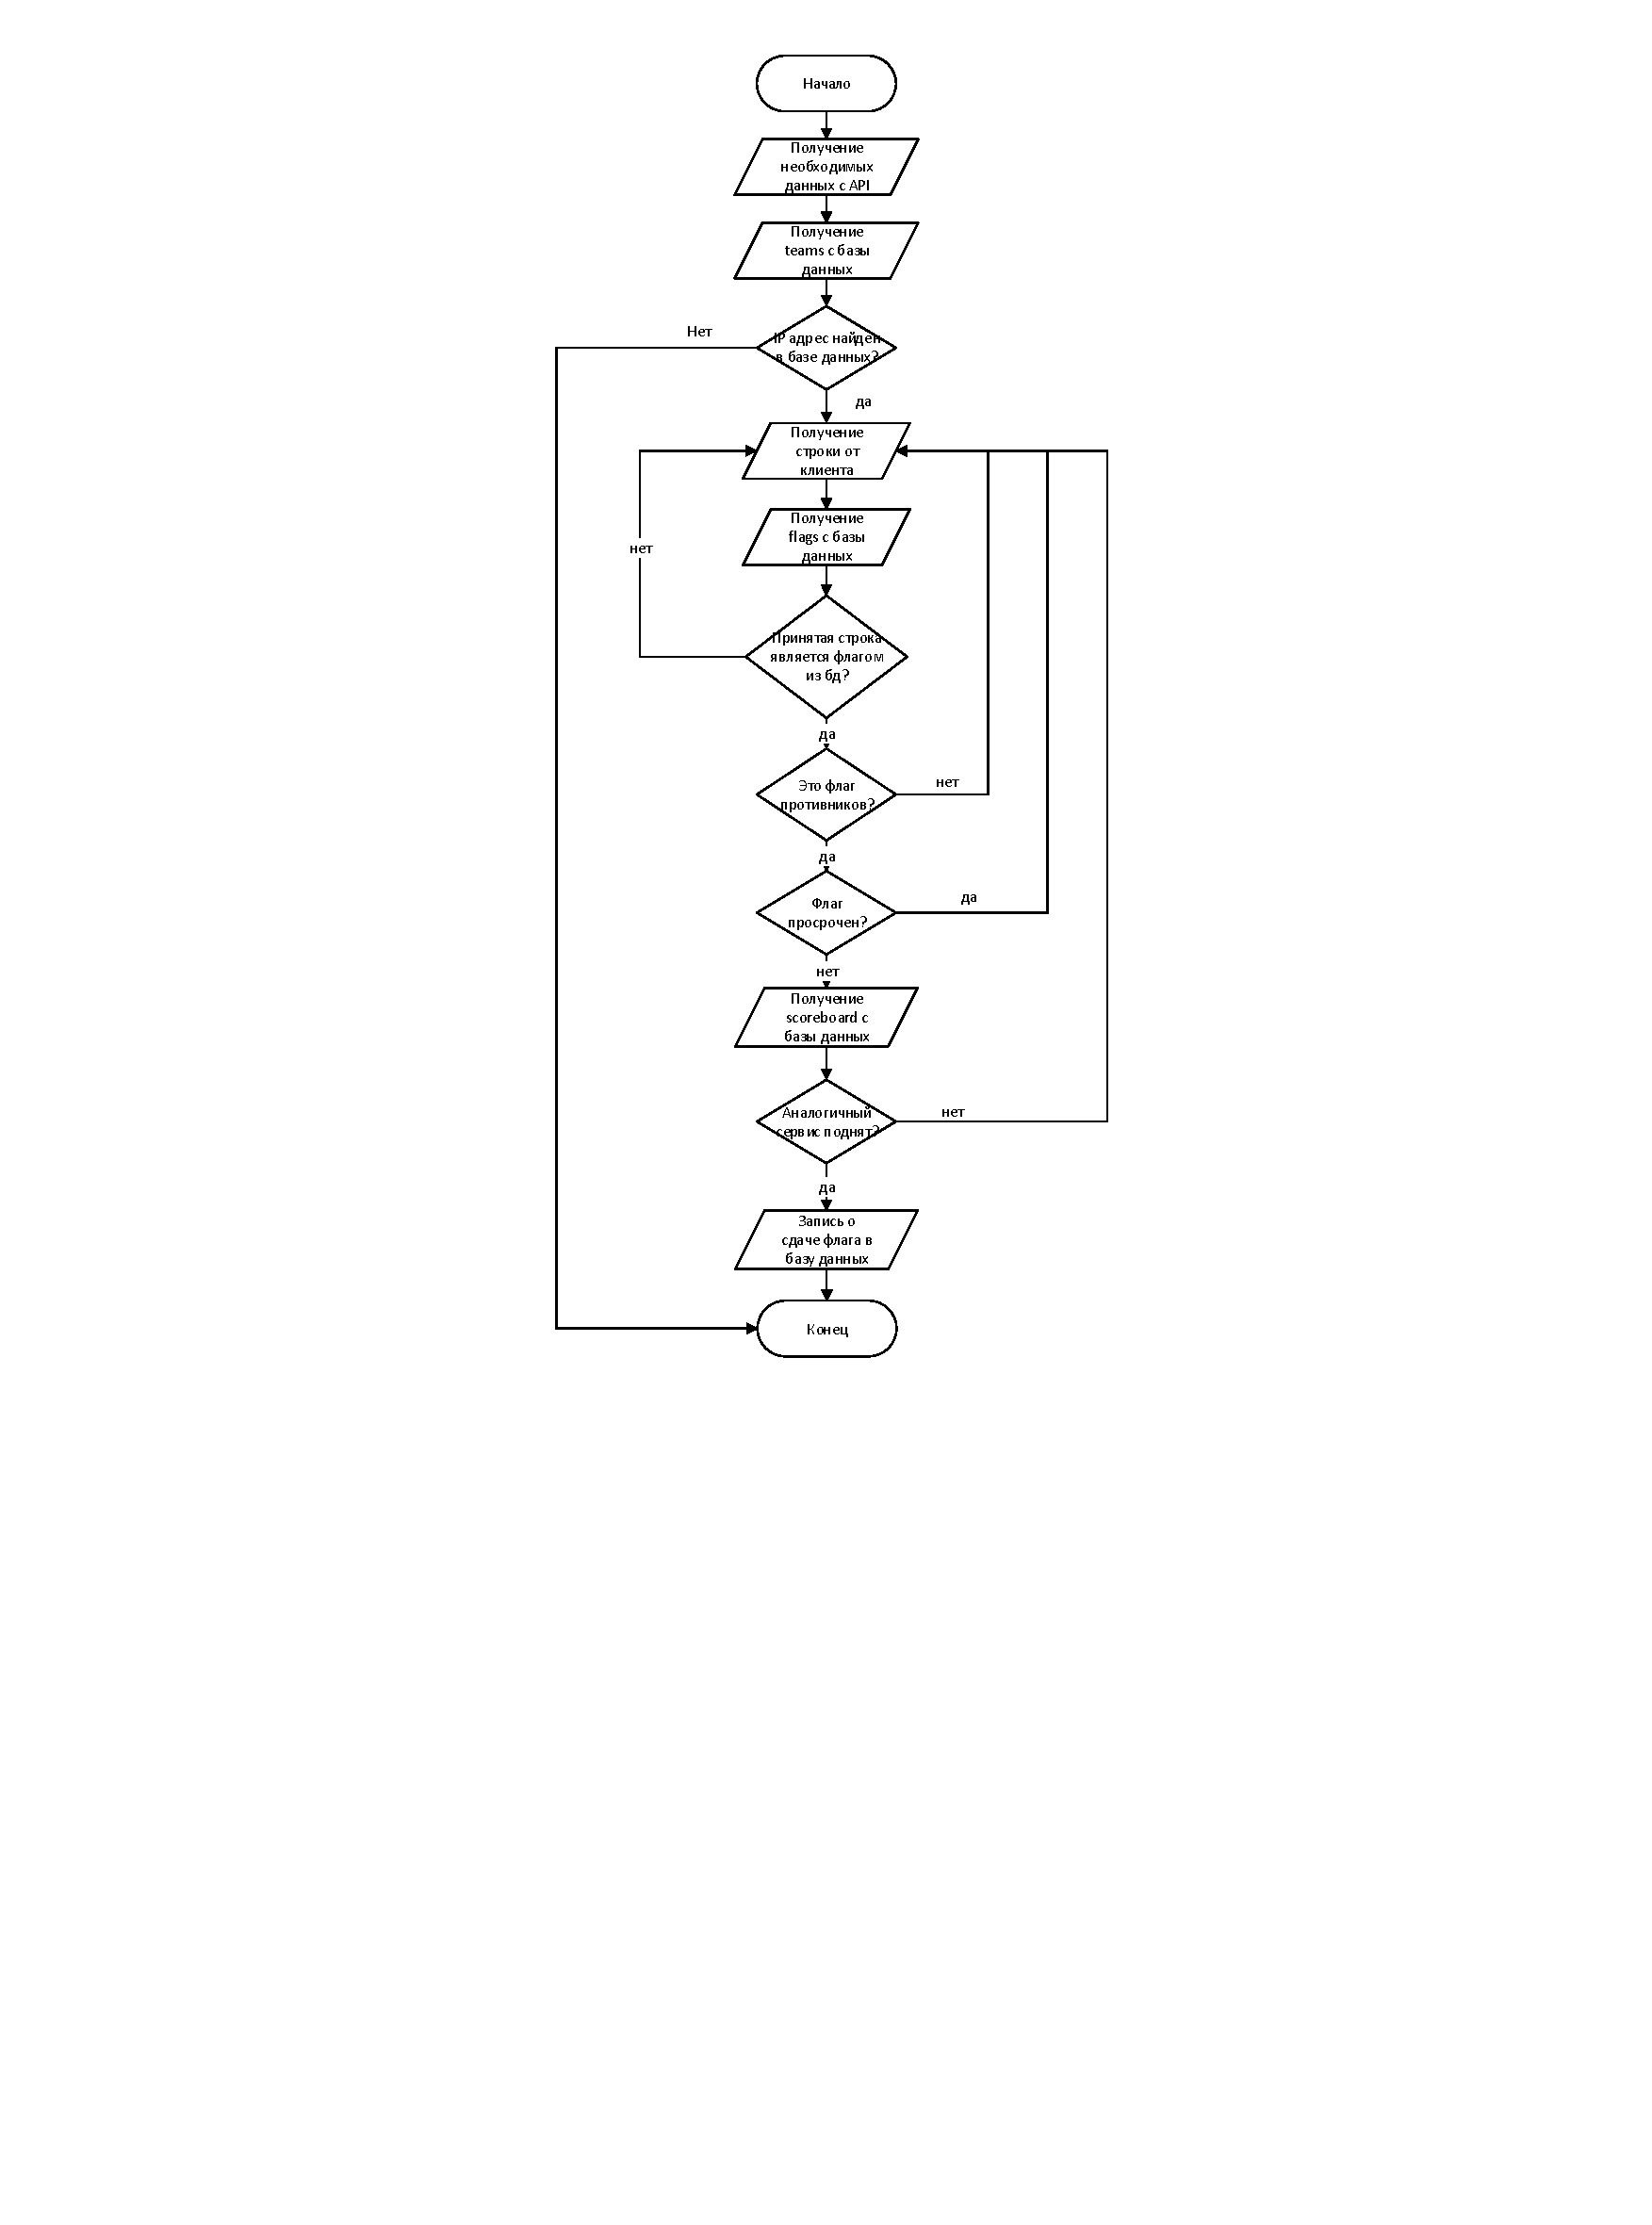
\includegraphics[trim=200 400 200 0, width=0.7\linewidth]{individual_reports/Algoritm.pdf}}
\caption{Алгоритм модуля flags.py}
\end{figure} 

\begin{figure}[h!]
\center{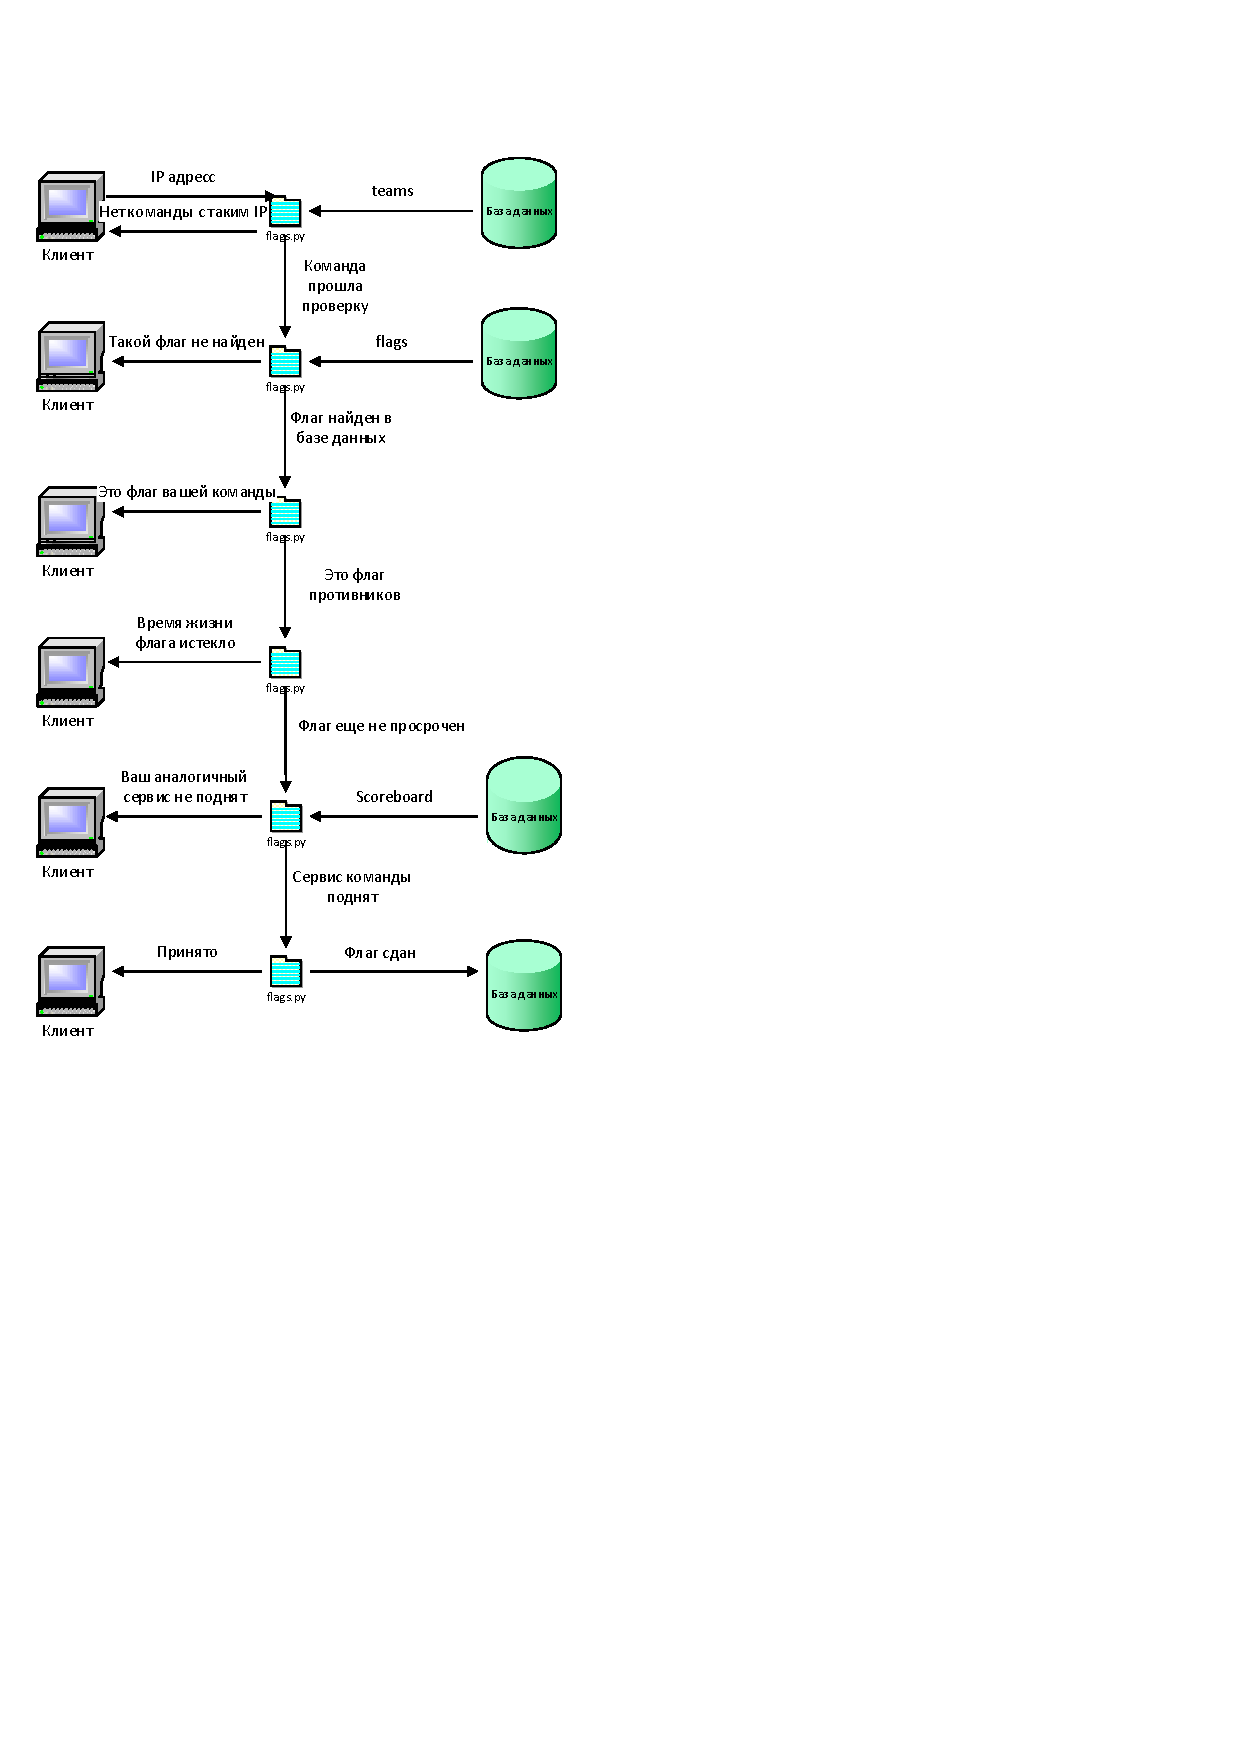
\includegraphics[trim=0 300 300 0, width=0.7\linewidth]{individual_reports/Naglyadno.pdf}}
\caption{Наглядная схема работы flags.py}
\end{figure} 

\clearpage